% template created by: Russell Haering. arr. Joseph Crop
\documentclass[12pt,letterpaper]{article}
\usepackage{anysize}
\usepackage{cite}
\usepackage{amsmath,amssymb,amsfonts}
\usepackage{algorithm}
\usepackage[noend]{algpseudocode}
\usepackage{graphicx}
\usepackage{multirow}
\usepackage{listings}
\usepackage{xcolor}


\marginsize{2cm}{2cm}{1cm}{1cm}

\lstset{ framexleftmargin=9mm, frame=shadowbox,tabsize = 4}

\begin{document}

\begin{titlepage}
    \vspace*{4cm}
    \begin{flushright}
    {\huge
        ECE 375 Lab 5\\[1cm]
    }
    {\large
    	External Interrupts
    }
    \end{flushright}
    \begin{flushleft}
    Lab session: 015
    
    Time: 12:00-13:50
    \end{flushleft}
    \begin{flushright}
    Author: Astrid Delestine

    Programming partner: Lucas Plastid 

    \vfill
    \rule{5in}{.5mm}\\
    TA Signature
    \end{flushright}

\end{titlepage}

\section{Introduction}
%This is the first Lab in the ECE 375 series and it covers the setup and compilation of an AVR Assembly Program. The student will learn how how to use the sample Basic Bump Bot assembly file and send the binaries to the AVR Microcontroller board. For the second part of the lab the student will be expected to download and compile the included C sample program and from it learn how to configure the I/O ports of the ATmega32U4 Microcontroller. The student will then write their own C program and upload it to the Microcontroller to verify that it runs as expected. The provided programs have been attached in the source code section of this report.
This is the Fifth lab in the ECE 375 series and it covers using hardware interrupts to preform predescribed "bump bot" operations. Additionally it incorporated use of the LCD Display to show the user how many times the bump bot had been triggered on its left or right side

\section{Design}
In this lab Lucas and I setup several different interrupt vectors that were able to trigger certain functions. These functions made the program function similarly to the Lab 1 and 2 bump bot script. Once these interrupts were created and working we moved to creating counters and displays for each of the buttons pressed. In the image seen below, one can see an example of what the LCD display would look like upon boot up. 

\begin{figure}[h]
	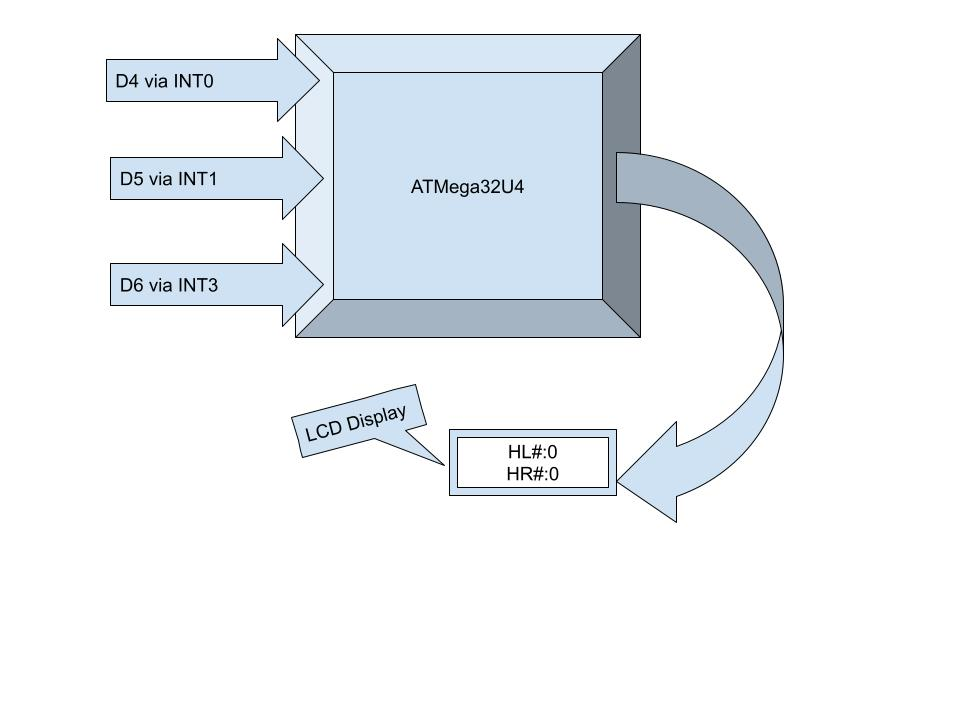
\includegraphics[width=12cm, height=10cm]{Block Diagram L5.jpg}
	\centering
\end{figure}
	
\section{Assembly Overview}
As for the Assembly program an overview can be seen below. 

\subsection{Internal Register Definitions and Constants}
The multipurpose register was setup as r16. At r0 and r1 any multiplication output will be set, such that the outputs of any multiplication operation are automatically assigned to them. A default zero register is set to r2. Two other generic variable registers are defined as r3 and r4. Finally two registers named oloop and iloop are used for counting within the assembly itself.

\subsection{Interrupt Vectors}
Vectors setup are;
hit right on interrupt 0,
hit left on interrupt 1,
and clear counters on interrupt 3.



\subsection{Initialization Routine}
Firstly the stack pointer is initialized then ports B and D are initialized for output and input respectively. The LCD is then initialized in its own subroutines as we set it to turn its backlight on and clear any remaining text on the screen. Then we set it such that it displays clear delimiters for each of our button presses. Next we load up the interrupt control for falling edge detection, and configure the interrupt mask for just the 3 interrupts we had setup earlier. Finally we run the sei command to set the interrupt flag in SREG so that the interrupts can work at all.

\subsection{Main Routine}
The main routine is very simple due to the fact that most operations are handled outside of the main routine by interrupts. 


\subsection{Subroutines}
	\subsection{ClearCounters}
	This subroutine clears the counters for each button press, then clears the LCD of any overflowing numbers, and resets it back to its initial state. This is done by loading all 16 characters into the data memory that the display looks at for its characters.  
	
	\subsection{toLCD}
	The toLCD subroutine is quite simple with regards to what we have already completed. It sets the first four bits of each row to the characters in data memory then uses the built in Bin2ASCII command to take the mpr register and print it to the LCD display. It then enables the LCD to write the characters to the screen.

	\subsubsection{HitRight}
	This subroutine takes 4 different data locations and multiplies 24 bits by 24 bits, resulting in a 48 bit number. It must be built differently to the MUL16 operation. Every time addition occurs  we need to check for the carry bit and pass it forward if necessary. This will continue until there is no carry bit to pass upward. In reality this can only ever happen up to 4 times. In this subroutine the first operand is loaded into the Z pointer. Then the second operand is loaded into the Y pointer, finally the result is loaded into the X register. For each of these, they load the start of each because they will increment throughout the method. The data in Y an Z are multiplied and the result is stored in r0 and r1. ADDMUL2x is then called. This fixes the carry bit problem of multiplying by 24 bits and as long as we call ADDMUL2x after our multiplication then everything will work out. 
	 
	
	\subsubsection{HitLeft}
	This subroutine adds a partial multiplication result to the location x is pointing to. This presumes that x is already pointing to the location where the low result of the current multiplication needs to go. Essentially it takes the multiplication outputs and cycles the carry bit up until it cannot anymore. It utilized a loop moving the carry byte in and out of X when necessary.
	
	\subsubsection{Wait}
	Preforms the operation \(((G-H)+I)^2\) Using multiplication, addition and subtraction.
	

\section{Testing}
Tested Each input value and compared to external calculations.
\begin{table}[h]
	\centering
	\begin{tabular}{|l|l|l|ll}
		\cline{1-3}
		Case & Expected & Actual meet expected &  &  \\ \cline{1-3}
	\( \$FCBA + \$FFFF \) 	&\$01FCB9&	\checkmark  &  \\ \cline{1-3}
	\( \$FCB9 - \$E420 \)	&\$1899&	\checkmark	&  \\ \cline{1-3}
	\( \$00FFFFFF * \$00FFFFFF \)	&\$FFFFFE000001&	\checkmark  &  \\ \cline{1-3}
	\(((\$FCBA-\$2022)+\$21BB)^2\)	&\$FCA8CEE9&	\checkmark	&  \\ \cline{1-3}
	
%		&          &                      &  &  \\ \cline{1-3}
	\end{tabular}
\caption{Assembly Testing Cases}
\end{table}

\section{Study Questions}
\begin{enumerate}
    \item
    As this lab, Lab 1, and Lab 2 have demonstrated, there are always multiple ways to accomplish the same task when programming (this is especially true for assembly programming). As an engineer, you will need to be able to justify your design choices. You have now seen the BumpBot behavior implemented using two different programming languages (AVR assembly and C), and also using two different methods of receiving external input (polling and interrupts).
    Explain the benefits and costs of each of these approaches. Some important areas of interest include, but are not limited to: efficiency, speed, cost of context switching, programming time, understandability, etc.
    
    
    \item 
    Instead of using the Wait function that was provided in BasicBumpBot.asm, is it possible to use a timer/counter interrupt to perform the one-second delays that are a part of the BumpBot behavior, while still using external
    interrupts for the bumpers? Give a reasonable argument either way, and be sure to mention if interrupt priority had any effect on your answer.
    
    
    \item 
    List the correct sequence of AVR assembly instructions needed to store the contents of registers R25:R24 into Timer/Counter1’s 16-bit register, TCNT1. (You may assume that registers R25:R24 have already been initialized to contain some 16-bit value.
    
 	
    (because its an IO location)
    out TCNT1H r25
    out TCNT1L r24
    
    \item
    List the correct sequence of AVR assembly instructions needed to load the contents of Timer/Counter1’s 16-bit register, TCNT1, into registers R25:R24
    
    in r25 TCNT1H
    in r24 TNCT1L
    
    \item 
    Suppose Timer/Counter0 (an 8-bit timer) has been configured to operate in Normal mode, and with no prescaling (i.e., clkT 0 = clkI/O = 8 MHz). The decimal value “128” has just been written into Timer/Counter0’s 8-bit
    register, TCNT0. How long will it take for the TOV0 flag to become set? Give your answer as an amount of time, not as a number of cycles
    
    it will take 16 microseconds
    
    
\end{enumerate}

\section{Difficulties}
This lab was more challenging than the last, however it did not require us to learn anything outside of lecture. This is a good thing, due to the fact that we re only expected to know exactly what we are taught.

\section{Conclusion}
This lab cemented the ideas of logical operands and allowed the student to understand how computers operate with large numbers, especially larger numbers than they might be able to handle naively. Additionally the pencil and paper method described in the handout was not how I was taught how to do multiplication, so the solution may be more or less difficult depending on the students type of education.

\pagebreak

\section{Source Code}%
\lstinputlisting
[
caption=Assembely Bump Bot Script,
language={[x86masm]Assembler},
numbers =left,
rulesepcolor=\color{blue}
]{../Lab5Assm/Lab5Assm/Lab5Assm/Astrid_Delestine_and_Lucas_Plaisted_Lab5_sourcecode.asm}





\end{document}